\documentclass[border=2pt]{standalone}
\usepackage{fontspec}
\setmainfont{TeX Gyre Pagella}
\usepackage{pgfplots}
\pgfplotsset{compat=1.18}
\usepackage{amsmath}
\begin{document}
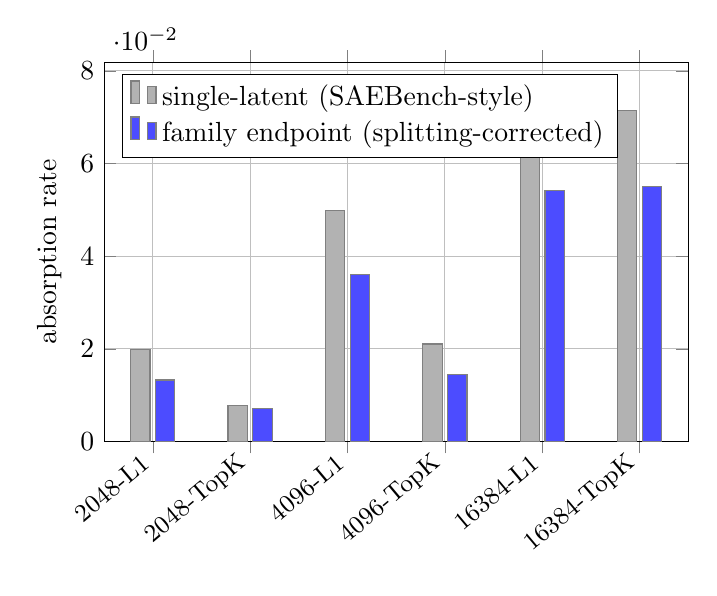
\begin{tikzpicture}
\begin{axis}[width=9cm,height=6.4cm,ybar,bar width=7pt,
  symbolic x coords={2048-L1,2048-TopK,4096-L1,4096-TopK,16384-L1,16384-TopK},
  xtick=data,x tick label style={rotate=40,anchor=east,font=\small},
  ylabel={absorption rate},legend pos=north west,legend cell align=left,
  grid=major,ymin=0]
\addplot[fill=gray!60,draw=black!50] coordinates {(2048-L1,0.01989) (2048-TopK,0.00775) (4096-L1,0.04984) (4096-TopK,0.02106) (16384-L1,0.07444) (16384-TopK,0.07146)};
\addlegendentry{single-latent (SAEBench-style)}
\addplot[fill=blue!70,draw=black!50] coordinates {(2048-L1,0.01328) (2048-TopK,0.00713) (4096-L1,0.03606) (4096-TopK,0.01449) (16384-L1,0.05422) (16384-TopK,0.05509)};
\addlegendentry{family endpoint (splitting-corrected)}
\end{axis}
\end{tikzpicture}
\end{document}
